\documentclass[border=4pt]{standalone}
\usepackage[utf8]{inputenc}\usepackage[T1]{fontenc}\usepackage{mathptmx}
\usepackage{tikz}\usetikzlibrary{positioning,arrows.meta,calc,fit}
\begin{document}
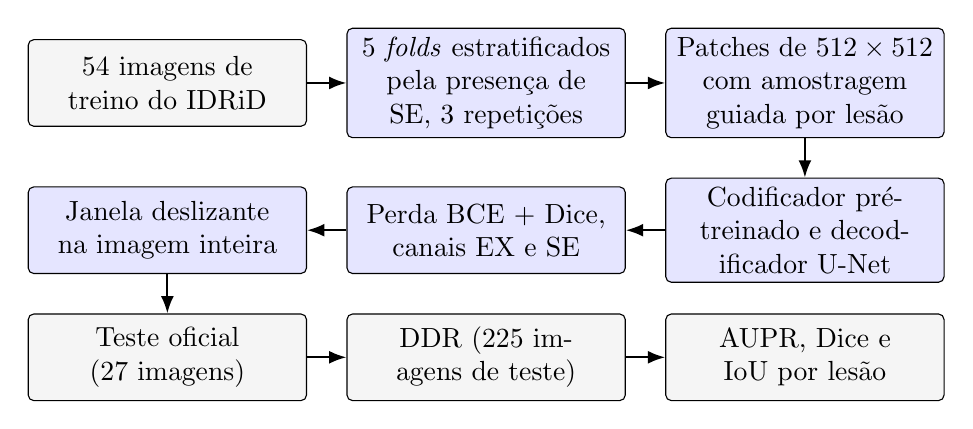
\begin{tikzpicture}[font=\normalsize,node distance=0.5cm and 0.5cm,
  b/.style={draw,rounded corners=2pt,align=center,text width=3.3cm,minimum height=1.1cm,fill=blue!10},
  g/.style={draw,rounded corners=2pt,align=center,text width=3.3cm,minimum height=1.1cm,fill=gray!8},
  arr/.style={-{Latex[length=2.2mm]},thick}]
\node[g] (a) {54 imagens de treino do IDRiD};
\node[b,right=of a] (b) {5 \textit{folds} estratificados pela presença de SE, 3 repetições};
\node[b,right=of b] (c) {Patches de $512\times512$ com amostragem guiada por lesão};
\node[b,below=of c] (d) {Codificador pré-treinado e decodificador U-Net};
\node[b,left=of d] (e) {Perda BCE + Dice, canais EX e SE};
\node[b,left=of e] (f) {Janela deslizante na imagem inteira};
\node[g,below=of f] (g) {Teste oficial (27 imagens)};
\node[g,right=of g] (h) {DDR (225 imagens de teste)};
\node[g,right=of h] (i) {AUPR, Dice e IoU por lesão};
\draw[arr] (a)--(b); \draw[arr] (b)--(c); \draw[arr] (c)--(d); \draw[arr] (d)--(e); \draw[arr] (e)--(f);
\draw[arr] (f)--(g); \draw[arr] (g)--(h); \draw[arr] (h)--(i);
\end{tikzpicture}
\end{document}
